\documentclass[10pt,a4paper]{article}
\usepackage[utf8]{inputenc}
\usepackage[T1]{fontenc}
\usepackage{amsmath}
\usepackage{amsfonts}
\usepackage{amssymb}
\usepackage{graphicx}
\usepackage{hyperref}
\usepackage{pdfpages}
\author{Andrew Rosen}
\title{Proposal \\ Data Structures}
\date{}
\begin{document}
	
\maketitle

\begin{enumerate}
	\item My aim is to replace the current textbook used in CIS 2168 (Data Structures) with a free resource the students can utilize. 
	Data Structures is one of the fundamental topics in Computer Science and is taught in some form at \emph{every} school that offers a Computer Science degree. 
	Furthermore, it is one of the two courses (the other being the Algorithms course) around which large tech companies tailor the content of technical interviews.  
	Students are stretched for cash as it is and additional costs of textbooks can serve as both a real and perceived barrier to entry.
	Additionally, I want to host this project on GitHub so that other instructors can create their own version of the textbook and make additional contributions to the text. 
	\item\href{https://github.com/abrosen/DataStructuresTextbook}{You can view my progress on the textbook by clicking this sentence.} 
	You can find the current table of contents attached.
	\item The target audience at Temple is all students required to take CIS 2168, which is every student enrolled in the CIS or IST major or minor program.  This is about 175 students a semester.  This course is required in some fashion at all universities that offer a computer science degree. Data Structures is sometimes referred to as CS2, where CS1 would be the intro to programming course.  There is some variation among universities as to which course gets which specific topic, but that is more a matter of timing than anything else.  This is a roundabout way of saying that this book is applicable to any student getting a CS or CS related degree who has taken their introductory programming courses.  
	\item We currently use ``Data Structures: Abstraction and Design Using Java'' by Koffman and Wolfgang, which costs ~\$125.  Other textbooks for this course exist, such as Prichard and Carrano’s ``Data Abstraction and Problem Solving with Java: Walls and Mirrors'' for a comparable price.  As mentioned above, every university that grants CS degrees teaches the topics in this course.  It is a required part of the CS curriculum and is offered every semester at every university I’ve been to.
	\item \href{https://faculty.washington.edu/ajko/cer}{Dr. Amy J. Ko keeps a list of Professors who do research in Computer Science education (Computing Education Research)}  many of these people would be good potential reviewers.  Other, more specific people I can reach out to: 
	\begin{enumerate}
		\item \href{https://people.cs.vt.edu/~shaffer/}{Cliff Shafer}
		\item \href{https://drexel.edu/cci/about/directory/P/Pirmann-Tammy/}{Tammy Pirmann}
		\item \href{https://www.unomaha.edu/college-of-information-science-and-technology/about/faculty-staff/briana-morrison.php}{Brianna Morrison}
		\item \href{https://acbart.github.io/}{Austin Cory Bart}
		\item \href{https://www.cc.gatech.edu/people/melinda-mcdaniel}{Melinda McDaniel}
		
	\end{enumerate}
	 
\end{enumerate}	

\includepdf[pages={3-5}]{textbook.pdf}

\end{document}